\subsection{premi/client/presentation}
\begin{figure}[h]
\begin{center}
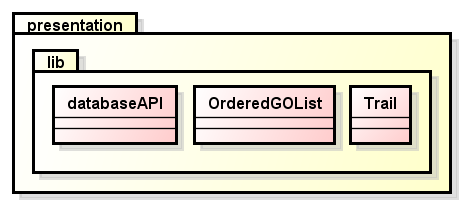
\includegraphics[scale=0.90]{img/diapkg/presentation.png}
\caption{Diagramma del package premi/client/presentation}
\end{center}
\end{figure}


%-------  diagramma della classe%
\subsubsection{premi/client/presentation/lib/databaseAPI}
\begin{figure}[h]
\begin{center}
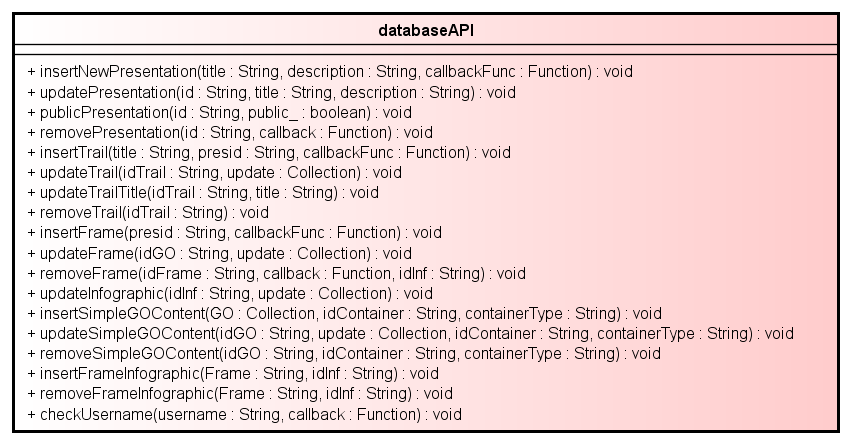
\includegraphics[scale=0.55]{img/diacla/databaseAPI.png}
\caption{Diagramma della classe premi/client/presentation/lib/databaseAPI}
\end{center}
\end{figure}


\begin{description}
%-------  descrizione della classe%
\item[Descrizione] \hfill \\
	Classe di metodi statici che permette al client di interfacciarsi ai metodi corrispondenti del server
	
	
%-------  lista dei metodi%	
\item[Metodi] \hfill \\

	% -- inizio metodo -- %
	\begin{description}
		\item[\textbf{\color{blue}+ insertNewPresentation(title : String, description : String, callbackFunc : Function) : void			}] \hfill \\
			Permette l'inserimento di una nuova presentazione all'interno del database
			
		\begin{description}
			% -- lista argomenti del metodo -- %
			\item[Argomenti] \hfill \\
				\begin{itemize}
				
					\item \textbf{title : String			} \hfill \\
					Titolo della nuova presentazione
					\item \textbf{description : String			} \hfill \\
					Descrizione della nuova presentazione
					\item \textbf{callbackFunc : Function			} \hfill \\
					Funzione di callback$_G$ per la restituzione dell'id della presentazione
					
				\end{itemize}
			% -- note aggiuntive sul metodo -- %
			\item[Note] \hfill \\
			\begin{itemize}
					\item Chiama il metodo \textit{insertPresentation} pubblicato in \textit{\$meteor}
			\end{itemize}
		\end{description}
	\end{description}
	% -- fine metodo -- %		



	% -- inizio metodo -- %
	\begin{description}
		\item[\textbf{\color{blue}+ updatePresentation(id : String, title : String, description : String) : void			}] \hfill \\
			Permette l'aggiornamento del titolo e della descrizione di una presentazione dell'utente
			
		\begin{description}
			% -- lista argomenti del metodo -- %
			\item[Argomenti] \hfill \\
				\begin{itemize}
					\item \textbf{id : String			} \hfill \\
					Codice identificativo della presentazione da aggiornare
					\item \textbf{title : String			} \hfill \\
					Nuovo titolo della presentazione
					\item \textbf{description : String			} \hfill \\
					Nuova descrizione della presentazione
					
				\end{itemize}
			% -- note aggiuntive sul metodo -- %
			\item[Note] \hfill \\
			\begin{itemize}
					\item Chiama il metodo \textit{editPresentation} pubblicato in \textit{\$meteor}
			\end{itemize}
		\end{description}
	\end{description}
	% -- fine metodo -- %		


	% -- inizio metodo -- %
	\begin{description}
		\item[\textbf{\color{blue}+ publicPresentation(id : String, public\_ : boolean) : void			}] \hfill \\
			Rende una presentazione pubblica o privata
			
		\begin{description}
			% -- lista argomenti del metodo -- %
			\item[Argomenti] \hfill \\
				\begin{itemize}
					\item \textbf{id : String			} \hfill \\
					Codice identificativo della presentazione da aggiornare
					\item \textbf{public\_ : boolean			} \hfill \\
					Variabile booleana: se \textit{true} la presentazione verrà resa pubblica, se \textit{false} verrà resa privata
					
				\end{itemize}
			% -- note aggiuntive sul metodo -- %
			\item[Note] \hfill \\
			\begin{itemize}
					\item Chiama il metodo \textit{publicPresentation} pubblicato in \textit{\$meteor}
			\end{itemize}
		\end{description}
	\end{description}
	% -- fine metodo -- %		


	% -- inizio metodo -- %
	\begin{description}
		\item[\textbf{\color{blue}+ removePresentation(id : String, callback : Function) : void			}] \hfill \\
			Permette la rimozione di una presentazione dell'utente dal database
			
		\begin{description}
			% -- lista argomenti del metodo -- %
			\item[Argomenti] \hfill \\
				\begin{itemize}
					\item \textbf{id : String			} \hfill \\
					Codice identificativo della presentazione da rimuovere
					\item \textbf{callbackFunc : Function			} \hfill \\
					Funzione di callback$_G$ per la restituzione di una conferma dell'avvenuta rimozione della presentazione
					
				\end{itemize}
			% -- note aggiuntive sul metodo -- %
			\item[Note] \hfill \\
			\begin{itemize}
					\item Chiama il metodo \textit{removePresentation} pubblicato in \textit{\$meteor}
			\end{itemize}
		\end{description}
	\end{description}
	% -- fine metodo -- %		



	% -- inizio metodo -- %
	\begin{description}
		\item[\textbf{\color{blue}+ insertTrail(title : String, presid : String, callbackFunc : Function) : void			}] \hfill \\
			Permette l'inserimento di un trail all'interno del database
			
		\begin{description}
			% -- lista argomenti del metodo -- %
			\item[Argomenti] \hfill \\
				\begin{itemize}
					\item \textbf{title : String			} \hfill \\
					Titolo del trail da inserire
					\item \textbf{presid : String			} \hfill \\
					Codice identificativo della presentazione associata al trail
					\item \textbf{callbackFunc : Function			} \hfill \\
					Funzione di callback$_G$ per la restituzione del codice identificativo del nuovo trail creato
					
				\end{itemize}
			% -- note aggiuntive sul metodo -- %
			\item[Note] \hfill \\
			\begin{itemize}
					\item Chiama il metodo \textit{insertTrail} pubblicato in \textit{\$meteor}
			\end{itemize}
		\end{description}
	\end{description}
	% -- fine metodo -- %		
	
	% -- inizio metodo -- %
	\begin{description}
		\item[\textbf{\color{blue}+ updateTrail(idTrail : String, update : Collection) : void			}] \hfill \\
			Permette l'aggiornamento di un trail
			
		\begin{description}
			% -- lista argomenti del metodo -- %
			\item[Argomenti] \hfill \\
				\begin{itemize}
					\item \textbf{idTrail : String			} \hfill \\
					Codice identificativo del trail da aggiornare
					\item \textbf{update :  Collection			} \hfill \\
					Collezione di MongoDB degli attributi aggiornati del trail
					
				\end{itemize}
			% -- note aggiuntive sul metodo -- %
			\item[Note] \hfill \\
			\begin{itemize}
					\item Chiama il metodo \textit{updateTrail} pubblicato in \textit{\$meteor}
			\end{itemize}
		\end{description}
	\end{description}
	% -- fine metodo -- %	
	
	% -- inizio metodo -- %
	\begin{description}
		\item[\textbf{\color{blue}+ updateTrailTitle(idTrail : String, title : String) : void			}] \hfill \\
			Permette la modifica del titolo di un trail
			
		\begin{description}
			% -- lista argomenti del metodo -- %
			\item[Argomenti] \hfill \\
				\begin{itemize}
					\item \textbf{idTrail : String			} \hfill \\
					Codice identificativo del trail da aggiornare
					\item \textbf{title : String			} \hfill \\
					Nuovo titolo del trail
					
				\end{itemize}
			% -- note aggiuntive sul metodo -- %
			\item[Note] \hfill \\
			\begin{itemize}
					\item Chiama il metodo \textit{updateTrailById} pubblicato in \textit{\$meteor}
			\end{itemize}
		\end{description}
	\end{description}
	% -- fine metodo -- %	
	
	% -- inizio metodo -- %
	\begin{description}
		\item[\textbf{\color{blue}+ removeTrail(idTrail : String) : void			}] \hfill \\
			Permette la rimozione di un trail dal database
			
		\begin{description}
			% -- lista argomenti del metodo -- %
			\item[Argomenti] \hfill \\
				\begin{itemize}
					\item \textbf{idTrail : String			} \hfill \\
					Codice identificativo del trail da rimuovere
					
				\end{itemize}
			% -- note aggiuntive sul metodo -- %
			\item[Note] \hfill \\
			\begin{itemize}
					\item Chiama il metodo \textit{removeTrailById} pubblicato in \textit{\$meteor}
			\end{itemize}
		\end{description}
	\end{description}
	% -- fine metodo -- %	
	
	% -- inizio metodo -- %
	\begin{description}
		\item[\textbf{\color{blue}+ insertFrame(presid : String, callbackFunc : Function) : void			}] \hfill \\
			Permette l'inserimento di un frame all'interno del database
			
		\begin{description}
			% -- lista argomenti del metodo -- %
			\item[Argomenti] \hfill \\
				\begin{itemize}
					\item \textbf{presid : String			} \hfill \\
					Codice identificativo della presentazione associata al nuovo frame
					\item \textbf{callbackFunc : Function			} \hfill \\
					Funzione di callback$_G$ per la restituzione del codice identificativo del nuovo frame
					
				\end{itemize}
			% -- note aggiuntive sul metodo -- %
			\item[Note] \hfill \\
			\begin{itemize}
					\item Chiama il metodo \textit{insertFrameByIdPres} pubblicato in \textit{\$meteor}
			\end{itemize}
		\end{description}
	\end{description}
	% -- fine metodo -- %	
	
	% -- inizio metodo -- %
	\begin{description}
		\item[\textbf{\color{blue}+ updateFrame(idGO : String, update : Collection) : void			}] \hfill \\
			Permette l'aggiornamento di un frame all'interno del database
			
		\begin{description}
			% -- lista argomenti del metodo -- %
			\item[Argomenti] \hfill \\
				\begin{itemize}
					\item \textbf{idGO : String			} \hfill \\
					Codice identificativo del frame da aggiornare
					\item \textbf{update : Collection			} \hfill \\
					Collezione di MongoDB di attributi aggiornati
					
				\end{itemize}
			% -- note aggiuntive sul metodo -- %
			\item[Note] \hfill \\
			\begin{itemize}
					\item Chiama il metodo \textit{editFrameById} pubblicato in \textit{\$meteor}
			\end{itemize}
		\end{description}
	\end{description}
	% -- fine metodo -- %	
	
	% -- inizio metodo -- %
	\begin{description}
		\item[\textbf{\color{blue}+ removeFrame(idFrame : String, callback : Function, idInf : String) : void			}] \hfill \\
			Permette la rimozione di un frame dal database
			
		\begin{description}
			% -- lista argomenti del metodo -- %
			\item[Argomenti] \hfill \\
				\begin{itemize}
					\item \textbf{idFrame : String			} \hfill \\
					Codice identificativo del frame da rimuovere
					\item \textbf{callback : Function			} \hfill \\
					Funzione di callback$_G$ per la restituzione del codice identificativo del frame
					
				\end{itemize}
			% -- note aggiuntive sul metodo -- %
			\item[Note] \hfill \\
			\begin{itemize}
					\item Chiama il metodo \textit{removeFrameInfographic} pubblicato in \textit{\$meteor} per rimuovere le associazioni del frame con l'infografica della presentazione
					\item Chiama il metodo \textit{removeFrameById} pubblicato in \textit{\$meteor} per rimuovere il frame dal database
			\end{itemize}
		\end{description}
	\end{description}
	% -- fine metodo -- %	
	
	% -- inizio metodo -- %
	\begin{description}
		\item[\textbf{\color{blue}+ updateInfographic(idInf : String, update : Collection) : void			}] \hfill \\
			Permette l'aggiornamento di un'infografica
			
		\begin{description}
			% -- lista argomenti del metodo -- %
			\item[Argomenti] \hfill \\
				\begin{itemize}
					\item \textbf{idInf : String			} \hfill \\
					Codice identificativo dell'infografica da aggiornare
					\item \textbf{update : Collection			} \hfill \\
					Collezione di MongoDB di attributi aggiornati
					
				\end{itemize}
			% -- note aggiuntive sul metodo -- %
			\item[Note] \hfill \\
			\begin{itemize}
					\item Chiama il metodo \textit{updateInfographicById} pubblicato in \textit{\$meteor}
			\end{itemize}
		\end{description}
	\end{description}
	% -- fine metodo -- %	
	
	% -- inizio metodo -- %
	\begin{description}
		\item[\textbf{\color{blue}+ insertSimpleGOContent(GO : Collection, idContainer : String, containerType : String) : void			}] \hfill \\
			Inserisce un oggetto grafico all'interno del database
			
		\begin{description}
			% -- lista argomenti del metodo -- %
			\item[Argomenti] \hfill \\
				\begin{itemize}
					\item \textbf{GO : Collection			} \hfill \\
					Collezione degli attributi dell'oggetto grafico
					\item \textbf{idContainer : String			} \hfill \\
					Codice identificativo del contenitore in cui inserire l'oggetto grafico
					\item \textbf{ContainerType : String			} \hfill \\
					Tipo del contenitore: puo' essere un frame(\textit{"frame})) o un'infografica (\textit{"infographic"})
					
				\end{itemize}
			% -- note aggiuntive sul metodo -- %
			\item[Note] \hfill \\
			\begin{itemize}
					\item Chiama il metodo \textit{insertGOContentFrame} pubblicato in \textit{\$meteor} se il contenitore è un frame, mentre chiama il metodo \textit{insertGOContentInfographic} se il contenitore è un'infografica
			\end{itemize}
		\end{description}
	\end{description}
	% -- fine metodo -- %	
	
		% -- inizio metodo -- %
	\begin{description}
		\item[\textbf{\color{blue}+ updateSimpleGOContent(idGO : String, update : Collection, idContainer : String, containerType : String) : void			}] \hfill \\
			Aggiorna un oggetto grafico con gli attributi modificati dall'utente
			
		\begin{description}
			% -- lista argomenti del metodo -- %
			\item[Argomenti] \hfill \\
				\begin{itemize}
					\item \textbf{idGO : String			} \hfill \\
					Codice identificativo dell'oggetto grafico da aggiornare
					\item \textbf{update : Collection			} \hfill \\
					Collezione di MongoDB di attributi aggiornati
					\item \textbf{idContainer : String			} \hfill \\
					Codice identificativo del contenitore in cui l'oggetto grafico è stato inserito
					\item \textbf{ContainerType : String			} \hfill \\
					Tipo del contenitore: puo' essere un frame(\textit{"frame})) o un'infografica (\textit{"infographic"})
					
				\end{itemize}
			% -- note aggiuntive sul metodo -- %
			\item[Note] \hfill \\
			\begin{itemize}
					\item Chiama il metodo \textit{updateGOContentFrame} pubblicato in \textit{\$meteor} se il contenitore è un frame, mentre chiama il metodo \textit{updateGOContentInfographic} se il contenitore è un'infografica
			\end{itemize}
		\end{description}
	\end{description}
	% -- fine metodo -- %	
	
	% -- inizio metodo -- %
	\begin{description}
		\item[\textbf{\color{blue}+ removeSimpleGOContent(idGO : String, update : Collection, idContainer : String, containerType : String) : void			}] \hfill \\
			Aggiorna un oggetto grafico con gli attributi modificati dall'utente
			
		\begin{description}
			% -- lista argomenti del metodo -- %
			\item[Argomenti] \hfill \\
				\begin{itemize}
					\item \textbf{idGO : String			} \hfill \\
					Codice identificativo dell'oggetto grafico da aggiornare
					\item \textbf{update : Collection			} \hfill \\
					Collezione di MongoDB di attributi aggiornati
					\item \textbf{idContainer : String			} \hfill \\
					Codice identificativo del contenitore in cui l'oggetto grafico è stato inserito
					\item \textbf{ContainerType : String			} \hfill \\
					Tipo del contenitore: puo' essere un frame(\textit{"frame})) o un'infografica (\textit{"infographic"})
					
				\end{itemize}
			% -- note aggiuntive sul metodo -- %
			\item[Note] \hfill \\
			\begin{itemize}
					\item Chiama il metodo \textit{updateGOContentFrame} pubblicato in \textit{\$meteor} se il contenitore è un frame, mentre chiama il metodo \textit{updateGOContentInfographic} se il contenitore è un'infografica
			\end{itemize}
		\end{description}
	\end{description}
	% -- fine metodo -- %	
	
	% -- inizio metodo -- %
	\begin{description}
		\item[\textbf{\color{blue}+ removeSimpleGOContent(idGO : String, idContainer : String, containerType : String) : void			}] \hfill \\
			Rimuove un oggetto grafico da un frame o da un'infografica
			
		\begin{description}
			% -- lista argomenti del metodo -- %
			\item[Argomenti] \hfill \\
				\begin{itemize}
					\item \textbf{idGO : String			} \hfill \\
					Codice identificativo dell'oggetto grafico da rimuovere
					\item \textbf{idContainer : String			} \hfill \\
					Codice identificativo del contenitore in cui l'oggetto grafico è stato inserito
					\item \textbf{ContainerType : String			} \hfill \\
					Tipo del contenitore: puo' essere un frame(\textit{"frame})) o un'infografica (\textit{"infographic"})
					
				\end{itemize}
			% -- note aggiuntive sul metodo -- %
			\item[Note] \hfill \\
			\begin{itemize}
					\item Chiama il metodo \textit{removeGOContentFrame} pubblicato in \textit{\$meteor} se il contenitore è un frame, mentre chiama il metodo \textit{removeGOContentInfographic} se il contenitore è un'infografica
			\end{itemize}
		\end{description}
	\end{description}
	% -- fine metodo -- %	
	
	% -- inizio metodo -- %
	\begin{description}
		\item[\textbf{\color{blue}+ insertFrameInfographic(Frame : String, idInf : String) : void			}] \hfill \\
			Inserisce un frame all'interno di un'infografica
			
		\begin{description}
			% -- lista argomenti del metodo -- %
			\item[Argomenti] \hfill \\
				\begin{itemize}
					\item \textbf{Frame : String			} \hfill \\
					Codice identificativo del frame
					\item \textbf{idInf : String			} \hfill \\
					Codice identificativo dell'infografica
					
				\end{itemize}
			% -- note aggiuntive sul metodo -- %
			\item[Note] \hfill \\
			\begin{itemize}
					\item Chiama il metodo \textit{insertFrameInfographic} pubblicato in \textit{\$meteor}
			\end{itemize}
		\end{description}
	\end{description}
	% -- fine metodo -- %	
	
	% -- inizio metodo -- %
	\begin{description}
		\item[\textbf{\color{blue}+ removeFrameInfographic(Frame : String, idInf : String) : void			}] \hfill \\
			Rimuove un frame all'interno di un'infografica
			
		\begin{description}
			% -- lista argomenti del metodo -- %
			\item[Argomenti] \hfill \\
				\begin{itemize}
					\item \textbf{Frame : String			} \hfill \\
					Codice identificativo del frame
					\item \textbf{idInf : String			} \hfill \\
					Codice identificativo dell'infografica
					
				\end{itemize}
			% -- note aggiuntive sul metodo -- %
			\item[Note] \hfill \\
			\begin{itemize}
					\item Chiama il metodo \textit{removeFrameInfographic} pubblicato in \textit{\$meteor}
			\end{itemize}
		\end{description}
	\end{description}
	% -- fine metodo -- %	
	
	% -- inizio metodo -- %
	\begin{description}
		\item[\textbf{\color{blue}+ checkUsername(username : String, callback : Function) : void			}] \hfill \\
			Verifica la presenza di uno username nel database
			
		\begin{description}
			% -- lista argomenti del metodo -- %
			\item[Argomenti] \hfill \\
				\begin{itemize}
					\item \textbf{username : String			} \hfill \\
					Nome utente da cercare nel database
					\item \textbf{callback : Function			} \hfill \\
					Funzione callback$_G$ per confermare la presenza o l'assenza dello username nel database
					
				\end{itemize}
			% -- note aggiuntive sul metodo -- %
			\item[Note] \hfill \\
			\begin{itemize}
					\item Chiama il metodo \textit{checkUsername} pubblicato in \textit{\$meteor}. Restituisce una variabile booleana che andrà passata alla funzione callback$_G$
			\end{itemize}
		\end{description}
	\end{description}
	% -- fine metodo -- %	














\end{description}

